%-*- coding: utf-8 -*
%
\documentclass[a4paper,12pt,final]{article}
%
% import des differents packages
\usepackage[T1]{fontenc}
\usepackage[utf8]{inputenc}
\usepackage{lmodern}
%~ \usepackage{amsmath,amsfonts,amssymb} % extensions de l'ams pour les mathématiques
\usepackage{graphicx} % pour insérer images et pdf entre autres
\usepackage[french,english]{babel}
\usepackage{listings}
\usepackage{hyperref}
%
% pour régler les marges :
\usepackage[top=2.5cm,bottom=2.3cm,right=2cm,left=2cm]{geometry}
%
%
\newcommand{\reporttitle}{Émeric TOSI - Apprentissage 2015-2017} % Titre
\newcommand{\reportauthor}{Émeric \textsc{TOSI}} % Auteur
\newcommand{\reportsubject}{Architecte Logiciel pour le Programme API} % Sujet
\newcommand{\reportdate}{21 septembre 2017} % Date
%
\newcommand{\HRule}{\rule{\linewidth}{0.5mm}}
\setlength{\parskip}{1ex} % Espace entre les paragraphes
%
%
\hypersetup{
    pdftitle={\reporttitle},%
    pdfauthor={\reportauthor},%
    pdfsubject={\reportsubject}%
}
%
%pp
\begin{document}
    %
    %
\begin{titlepage}
    %
    \begin{center}
        %
        \begin{minipage}[t]{0.48\textwidth}
            \begin{flushleft}
                
\includegraphics [width=60mm]{images/UT3-logo.jpg} \\[0.5cm]
                    \textsc{Université Toulouse III - STRI}
            \end{flushleft}
        \end{minipage}
        %
        \begin{minipage}[t]{0.48\textwidth}
            \begin{flushright}
                
\includegraphics [width=30mm]{images/orange-logo.jpg} \\[0.5cm]
                \textsc{Orange}
            \end{flushright}
        \end{minipage} \\[6.5cm]
        %
        \textsc{\Large \reportsubject}\\[0.5cm]
        \HRule \\[0.4cm]
        %
        {\huge \bfseries \reporttitle}\\[0.4cm]
        \HRule \\[1.7cm]
        %
        \begin{minipage}[t]{0.3\textwidth}
            \begin{flushleft} \large
                \emph{Auteur :}\\
                \reportauthor
            \end{flushleft}
        \end{minipage}
        %
        \begin{minipage}[t]{0.6\textwidth}
            \begin{flushright} \large
                \emph{Responsables :} \\
                M.~Rahim \textsc{KACIMI} (tuteur universitaire)\\
                M.~Yan \textsc{DELCROIX} (tuteur en entreprise)
            \end{flushright}
        \end{minipage}
        %
        \vfill
        %
        {\large \reportdate}
    %
    \end{center}
%
\end{titlepage}

    \cleardoublepage % Dans le cas du recto verso, ajoute une page blanche si besoin
    %
    \selectlanguage{french}
\begin{abstract}

Ce mémoire relate mes deux années d'apprentissage au sein du groupe Orange au poste d'architecte logiciel dans le programme API.
Le travail de ce programme consiste à promouvoir la conception selon des méthodes orientées services dans le cycle de vie du système d'information de l'entreprise, principalement en suivant les concepts d'API REST.
Les problématiques de gestion des systèmes d'information sont le nerf de la guerre des multinationales et ce sont le cœur du travail des directions des systèmes d'informations.
Des styles d'architectures logiciels tels que le REST ou les micro-services permettent de concevoir et d'améliorer la qualité des systèmes d'information dans le but de réduire les risques et les coûts.
Cependant certaines contraintes freinent encore leur adoption et leur mise en place dans cette entreprise : les infrastructures actuelles ne permettent pas encore l'obtention de tous les gains de ces architectures lorsque ce ne sont pas directement les différentes personnes des projets qui rejettent ces nouveautés.
Ces styles d'architectures ne répondent pas à tous les besoins mais ils sont une base solide et prête à être améliorés dans la construction d'un système d'information complexe et pérenne.
De nouveaux concepts et de nouvelles architectures se basent directement sur celles-ci et étendent leurs fonctions pour répondre à de nouveaux besoins toujours plus forts de communications inter-services internes et externes aux entreprises.

\end{abstract}

%
\selectlanguage{english}
\begin{abstract}

This report presents my two year apprenticeship in Orange as a software architect for the API program.
The API program promotes new service oriented architectures to information systems, mostly REST API.
Main concerns in firms is information systems complexity and its ability to be upgrade, these are real business risks and costs.
Some architecture designs like REST or micro-services solve these issues by providing universal way to conceive simple and consistent application interfaces.
They are a good start to continue extending information systems while limiting its complexity sum.
Nowadays there is a trouble in Orange, there is problems with current infrastructure to support these new architectures and their advantages are not totally perceived.
New concepts and architectures based on actual ones are already available to improves further functions and gains from this base.
Main goal is yet to made information systems able to handle always more requests between services inside and outside of companies.

\end{abstract}

    \cleardoublepage
    %
    \tableofcontents % Table des matières
    \sloppy          % Justification moins stricte : des mots ne dépasseront pas des paragraphes
    \cleardoublepage
    %
    \section*{Remerciements}
\addcontentsline{toc}{section}{Remerciements}

En premier lieu, je remercie M. Yan \textsc{DELCROIX}, directeur du programme API dans le groupe Orange.
Il m'a supervisé, guidé dans mon travail, offert des opportunités uniques et m'a aidé à trouver des solutions pour avancer tout au long de cette alternance.

Je remercie aussi M. Rahim \textsc{KACIMI}, enseignant à l'université Toulouse III – Paul Sabatier et chercheur à l’IRIT.
En tant que tuteur universitaire, il a suivi pendant ces deux années mes avancés ainsi que mon blog et s'est assuré que mon alternance se déroulait parfaitement.

Je souhaite particulièrement remercier M. Laurent \textsc{DECHAMBE} (et son alternant M. Frédéric \textsc{LUCIANI} cette seconde année) pour notre partage de la salle S215, nos échanges et notre entraide dans la bonne humeur pendant ces deux ans.

J'adresse également mes remerciements à toutes les personnes que j’ai rencontrées pendant ces deux années d’apprentissage tant en entreprise qu'à l'université pendant ma formation.
Elles m'ont permis de découvrir énormément de nouveaux concepts et de savoir-faire et ainsi d'apprendre énormément en si peu de temps.

    \cleardoublepage
    %
    \section*{Introduction} % Pas de numérotation
\addcontentsline{toc}{section}{Introduction} % Ajout dans la table des matières

L'alternance permet d'allier études et mise en pratique en entreprise.
C'est une combinaison gagnante pour s'insérer rapidement dans la vie active et obtenir un premier emploi qualifié.

Ce contrat d'apprentissage d'une durée de deux ans a complété les deux années de formation universitaire de Master STRI\,\footnote{STRI : Systèmes de Télécommunication et Réseaux Informatiques}.
J'ai fait des démarches auprès de plusieurs entreprises par rapport aux postes dans lesquels je souhaitais développer des compétences.
Plusieurs offres positives se sont présentées, j'ai finalement choisi la multinationale : Orange.

Pendant ces deux années j'ai ainsi découvert le fonctionnement d'une grande entreprise : ce poste d'architecte logiciel est une fonction transverse dans l'entreprise.
Mon rapport établit le bilan du travail et des recherches effectuées pendant ces deux années.

    \cleardoublepage
    %
    \section{Orange et son système d'information}
\label{p1}

    \subsection{Le groupe Orange}

        \subsubsection{Présentation de l'entreprise}

        Le groupe Orange est un des principaux opérateurs de télécommunications dans le monde avec un chiffre d’affaire de 41 milliards d’euros et 155 000 employés au 31 décembre 2016, dont 96 000 en France.
        Présent dans 29 pays, le Groupe sert 263 millions de clients.
        Orange est également l’un des leaders mondiaux des services de télécommunications aux entreprises multinationales sous la marque Orange Business Services.
        En septembre 2017, Orange diversifie ses activités et lance une banque « 100 \% mobile », Orange Bank\,\up{\cite{orangebank}}.

        \subsubsection{Son histoire}

        En France, le premier réseau de télécommunication voit le jour en 1792.
        Il s’agit du réseau de télégraphie de Chappe.
        Puis viennent les inventions du télégraphe électrique et du téléphone.

        L’État français crée en 1879 un ministère des Postes et Télégraphes.
        Ce dernier récupère la téléphonie en 1889 et devient le ministère des PTT\,\footnote{PTT : Postes, Télégraphes et Téléphones} en 1923.

        Dans les années 1970, la France investit massivement dans le déploiement du réseau de téléphonie fixe.
        Parallèlement, elle met au point la commutation numérique, le minitel et la norme GSM\,\footnote{GSM : \foreignlanguage{english}{Global System for Mobile Communications}, norme numérique de seconde génération pour la téléphonie mobile.}.

        Le 1er janvier 1988, la direction générale des télécommunications est renommée France Télécom.
        Cette structure est dorénavant dotée d'une personnalité morale distincte de l'État et acquiert une autonomie financière.
        Elle lance en 1992 la première offre française de téléphonie mobile avec Itineris.

        En 1996, France Télécom devient une société anonyme dont l’État français est le seul actionnaire.
        Un an plus tard, le capital est ouvert au public.
        Aujourd’hui, l’État est encore le premier actionnaire avec une participation d’un peu plus de 20 \%.

        En 2000, France Télécom rachète, en pleine bulle Internet, l’opérateur mobile britannique Orange.
        L’éclatement de la bulle met un terme à cette période d’expansion et la dette supportée par le groupe devient si importante que l’entreprise perd 96 \% de sa valeur capitalistique.

        En 2013, France Télécom devient Orange.

        \subsubsection{Les activités d'Orange}

            \paragraph{Fixe, mobile et Internet haut débit}

            Cœur de métier historique du Groupe, Orange conçoit, développe et exploite des réseaux fixes et mobiles en Europe, Afrique et Moyen-Orient afin d’apporter à ses clients une connectivité sans cesse enrichie par les possibilités du haut et du très haut débit et les nouvelles technologies (ADSL, Fibre, 3G, 4G…).

            Orange a, au 30 juin 2017, 269 millions de clients grand public à travers le monde.

            \paragraph{Vente en gros}

            Grâce à l’étendue mondiale de ses réseaux, et notamment son implication dans la construction et l’exploitation de câbles sous-marins, Orange est un acteur majeur du marché de gros, développant des solutions adaptées aux besoins des opérateurs.
            À ce jour, l’entreprise possède 450 000 km de câble sous-marin, soit dix fois le diamètre de la Terre.

            \paragraph{Services de communications aux entreprises}

            Grâce à Orange Business Services et à ses entités spécialisées, Orange apporte aux entreprises de toutes tailles des services d’infrastructures, des services d’intégration et des solutions numériques couvrant l’ensemble de leurs besoins : collaborateurs, relation client, gestion de projets, sécurité …

            \paragraph{Contenus}

            Activité clé dans un contexte de convergence accélérée, Orange joue un rôle important dans les contenus afin de proposer les meilleurs services à ses clients (TV, VOD, cinéma, séries, musique, jeux...).
            L’entreprise est par exemple présent dans le capital de Deezer, une plateforme de streaming musical ainsi que dans celui de Dailymotion, plateforme de streaming vidéo.

            \paragraph{Territoires}

            Partout où le Groupe est présent, Orange est partenaire des collectivités, sachant que l’aménagement numérique des territoires, les usages et les services innovants sont devenus des enjeux critiques pour l’attractivité des territoires et leur dynamisme économique et social.
            Orange est le deuxième opérateur sur la production des RIP\,\footnote{RIP : Réseaux d’Initiative Publique pour le déploiement de la fibre dans les zones non rentables}.

            \paragraph{Objets connectés}

            Dans ce secteur d’avenir, Orange se positionne sur l’ensemble de la chaîne de valeur : distribution et connexion d’objets, ainsi que la fourniture de services à valeur ajoutée dans le domaine de la santé, du bien-être, de la maison connectée, etc...
            Ils développent par ailleurs des plateformes pour stocker et rendre intelligentes les données générées par les nouveaux écosystèmes.
            Orange est par ailleurs membre du comité LoRa Alliance qui promeut la technologie LoRa.

            \paragraph{Services financiers sur mobile}

            Sur cet axe de diversification stratégique, Orange poursuit son développement avec des services transactionnels comme Orange Money en Afrique, des solutions de paiement sans contact (Orange Cash) et une offre inédite de banque mobile avec Orange Bank dont la commercialisation est prévue pour septembre 2017.

        \subsubsection{Une présence internationale}

        \begin{figure}[!ht]
            \center
            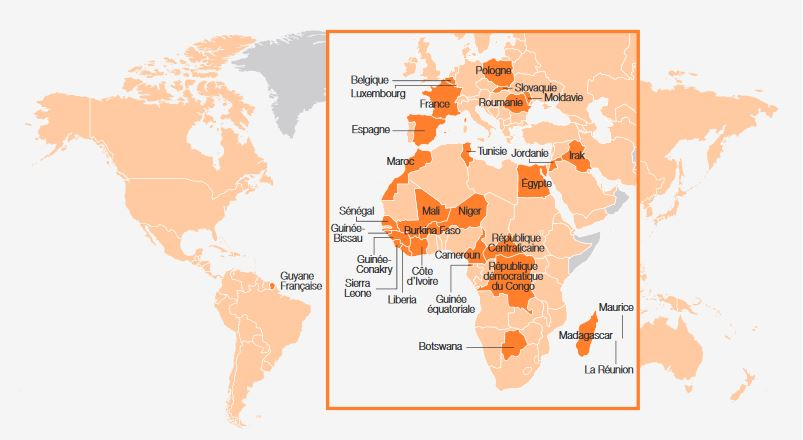
\includegraphics[width=1\textwidth]{./images/implem-mondiale-orange.jpg}
            \caption{Implantation mondiale d'Orange en 2017}
        \end{figure}

        Pour le grand public, l’entreprise est présente dans 29 pays sous la marque Orange avec 6 500 boutiques en nom propre.
        Sa zone de chalandise est l’Europe, l’Afrique et le Moyen-Orient.
        Néanmoins en terme de valeur, la France représente un peu moins de la moitié du chiffre d’affaires, quand l’Afrique et le Moyen-Orient constituent 12 \%.

        \subsubsection{Ses résultats financiers}

        \begin{figure}[!ht]
            \center
            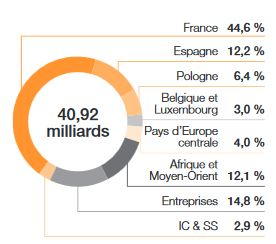
\includegraphics[width=0.4\textwidth]{./images/ca-orange.jpg}
            \caption{Chiffre d'affaires d'Orange Group en 2016}
        \end{figure}

        En 2016, Orange a généré un chiffre d’affaire de près de 41 milliards d’euros.
        L’entreprise en a tiré un résultat net de plus de 3 milliards d’euros et a distribué un dividende de 0,60 euros par action à ses actionnaires.

        \subsubsection{Les ressources humaines}

        Chez Orange se côtoie des fonctionnaires et des salariés sous contrat de droit privé.
        Les premiers sont issus des grandes vagues de recrutement du début des années 1980 pour faire face au retard de déploiement du réseau téléphonique.
        La privatisation de l’entreprise a généré chez eux des dégâts sociaux importants.
        Après des années de déni, la politique des ressources humaines s’est adaptée pour prendre en compte le bien être des salariés.
        Aujourd’hui Orange vise une proportion de 90 \% d’employés recommandant en tant qu’employeur en 2018.
        Fin 2016, ils étaient déjà 88 \% en France.
        Les fonctionnaires représentent encore une grande partie des salariés et sont proches de la retraite ce qui entraîne des départs à la retraite massifs.

        Orange emploie directement 155 000 personnes au 31 décembre 2016, dont 96 000 en France.
        L’entreprise est aussi engagée dans la formation avec le recrutement de 4 300 nouveaux alternants en 2016.

    \subsection{La DSI et ses objectifs}

    La Direction des Systèmes d’Information prend place au sein d’orange France.
    Elle œuvre au bon fonctionnement des différents systèmes d’information du groupe qui sont tous interconnectés pour former un SI\,\footnote{SI : Système d'information.} global.

    La principale mission de la DSI\,\footnote{DSI : Direction des systèmes d'information.} est l’uniformisation et l’évolution de ce SI global qui est un agrégat complexe, résultat des fusions et héritages des technologies commercialisées par le groupe.
    Ce SI est constitué de parties historiques et très hétérogènes ce qui représente une contrainte majeure dans sa maintenance et son fonctionnement tant sur le plan technique que sur le plan financier.
    La complexité du SI est un ensemble de risques, de coûts et de délais qu’il faut réussir à contrôler.

    Le groupe Orange adopte aujourd’hui une stratégie orienté vers les services, la santé et la réactivité de son système d’information sont donc cruciaux.
    La DSI est le cœur stratégique pour permettre au groupe de rester un acteur majeur dans la course à l’innovation et répondre aux attentes du marché d’aujourd’hui comme de demain.

    Une des missions perpétuelle au sein de la DSI est l’urbanisation du SI, cela consiste à  «cartographier» les différents processus métiers pour y répondre de la meilleure façon en diminuant les coûts d’exploitation associés.
    L’urbanisation est la transformation continue du SI pour rester cohérent avec les différents métiers et les stratégies du groupe.
    Cette démarche d’urbanisme permet la réduction des facteurs qui surviennent avec la complexité grandissante d’un système d’information.

    La direction des systèmes d’information est composé d’une entité pas branche métier du groupe ainsi qu’une entité globale qui s’occupent des projets qui portent sur l’ensemble du Si, de façon transverse à plusieurs domaines métiers.

    La DSI est en général la maîtrise d'ouvrage de l'informatique dans le groupe et parfois la maîtrise d'œuvre puisque elle est le centre de décision et l’initiateur des nouveaux projets pour le SI.
    Dans les autres cas la direction des systèmes d’information supervise les projets et est adjoint tant à la maîtrise d’œuvre qu’a la maîtrise d’ouvrage pour s’assurer du respects de ces directives et puisque le pôle architecture est une entité fille de la DSI.

    \subsection{Le pôle architecture et ses missions}

    Le pôle architecture est un centre de compétence de la direction des systèmes d’information.
    L’objectif d’un centre de compétences consiste à regrouper des connaissances : du savoir au savoir-faire autour d’une technologie, d’un outil ou d’une application.
    Selon le périmètre choisi, le centre de compétence interne pourra être responsable des études techniques et de l'intégration des nouveaux projets relatifs à son expertise, réaliser de la veille technologique, être l'interlocuteur de référence face aux intégrateurs et aux éditeurs, émettre de la documentation et formaliser le référentiel du projet, ou assurer le support et l'administration.

    Chez Orange, il existe par exemple un centre de compétence sur les environnements micro-services\,\footnote{Les micro-services sont un style d'architecture particulier se basant sur les API REST et où tout est découplé au maximum.}\,\up{\cite{microservices}} et l’application Docker\,\footnote{Docker est un logiciel plateforme de container, un container ressemble à une machine virtuelle allégée ne contenant que l'application souhaitée et ses dépendances.}\,\up{\cite{docker}} qui permettent une meilleure intégration des applications dans le SI.
    On trouve aussi un centre de compétence autour de la démarche Agile ou un autre plus vaste que les deux exemples précédents : le Pôle architecture, qui regroupe les différents architectes du groupe.

    Ces centres de compétences peuvent dépendre d’un domaine métier ou directement de la direction des systèmes d’information.
    Au sein d’Orange, l’appartenance d’un centre à une entité va dépendre de la manière dont elle a vu le jour.
    Les centres sont référencés dans le SI afin que les acteurs puissent les trouver et y faire appel de façon simple.

    La DSI contient donc le pôle architecture, un regroupement de plus de 600 personnes qui œuvrent au choix et stratégies à propos des applications et du système d’information du groupe.
    Le directeur de l’architecture du SI est Jean-Daniel Guedj qui manage donc ce centre de compétence.
    Le pôle architecture est le regroupement des personnes dont le travail est d’être référent sur les problématiques d’architecture logicielle, d’architecture fonctionnelle et d’architecture technique.

    Plusieurs missions et projets dont la portée est globale au niveau du groupe, et donc transverse à tous les domaines métiers, prennent place dans ce pôle architecture comme par exemple le programme api.

    \cleardoublepage
    %
    \section{Présentation du programme API et mon rôle dans celui-ci}
\label{p2}

    \subsection{Qu'est ce qu'une API ?}

    Le terme API\,\footnote{API : \foreignlanguage{english}{Application Programming Interface}, interface de programmation applicative en français.} est un terme générique identifiant une interface entre deux systèmes, notamment pour des interfaces temps réel web telles que les web-services.
    Attention toutefois, la démarche API et la démarche web-services sont différentes !

    Dans notre cas, une API est techniquement un web-service simple  accessible en self-service (au moins pour sa découverte) ;
    c’est-à-dire que des règles de design précises ont été respectées lors de sa conception (par ex. API REST\,\footnote{REST : \foreignlanguage{english}{Representational state transfer} , un style d'architecture basé sur le protocole HTTP.}\,\up{\cite{octodesign}}).
    Sa documentation est réalisée d’une façon particulière avec beaucoup de soin et un ensemble de bouchons sont disponibles pour réaliser des tests (l'équivalent d'un environnement bac à sable).

    \begin{figure}[!ht]
        \center
        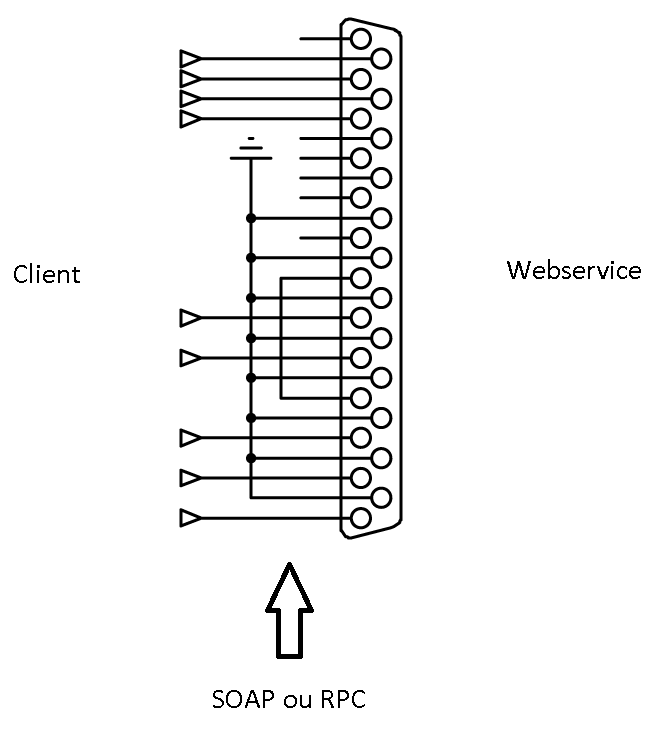
\includegraphics[width=0.5\textwidth]{./images/webservice.jpg}
        \caption{Un webservice typique offre de nombreux points d'entrée complexes}
    \end{figure}

    Le but de la démarche API est d’aller plus loin dans le découplage des applications et des organisations (projet notamment).
    Une API, c’est aussi un langage commun et transverse entre le métier et le SI.
    Résultat : une meilleure agilité, une simplicité et de meilleures performances pour le SI !

    Une API se construit grâce à une démarche commune de partage et de co-construction de tous les acteurs (fonctionnels comme techniques) en mettant dès le départ l'accent sur le design et la documentation.
    Une API est toujours construite dans l’optique qu’elle puisse être rendue publique, sa conception et son accessibilité doivent donc être le plus soignées possible.
    Contrairement aux web-services dotés d’un contrat d’interface complexe et différent pour chaque besoin client, les messages d’une API sont son interface qui lui est  unique, commune et globale.

    \begin{figure}[!ht]
        \center
        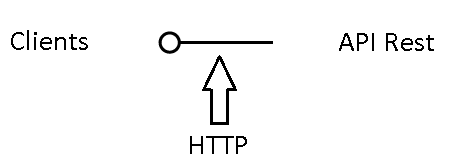
\includegraphics[width=0.35\textwidth]{./images/api-rest.jpg}
        \caption{Une API REST offre un point d'entrée unique et simple}
    \end{figure}

    Une API REST (representational state transfer) est une API client-serveur conçue grâce à une modélisation orientée ressources (et non plus méthodes comme c’était le cas en web-services) avec la contrainte d’être serveur sans état, c’est à dire que chaque message contient toutes les données et informations nécessaires à son traitement, il n’y a pas de contexte créé du coté serveur suite aux enchaînements de requêtes.
    Elle se base aussi sur un protocole de haut niveau omniprésent : HTTP, qui fournit des verbes (méthodes GET POST DELETE PUT ...) ainsi que le système de schéma (URL, URI), cela lui procure une facilité d’usage universelle.
    Nous parlerons maintenant d’API en tant qu’abréviation d’API REST.

    La question que les architectes et designers doivent se poser n’est pas
    “Comment un serveur doit-il exporter ses objets privés de sorte que les clients puissent les comprendre et les utiliser ? “, mais plutôt
    “Comment un client et un serveur peuvent partager une compréhension commune des données brutes échangées entre eux ?”\,\up{\cite{apihtml5}}

    Un client est donc autonome grâce à la simplicité et au self-service (catalogue d’API) ainsi que la robustesse des API induite par leur fort découplage.
    La documentation complète répond à la majorité de ces questions, il peut aussi contacter l’équipe projet pour exprimer ses demandes (demandes qui seront donc évaluées et peut-être ajoutées dans la documentation).

    Le fournisseur d’API l’expose sur une « Gateway », point d’accès et d’exposition central, et y délègue tout ou partie de la gestion des quotas clients.
    Il n’a donc pas à configurer pour chaque client l’interconnexion, le processus est automatisé au maximum possible (en gardant les spécificités métiers s’il y en a).
    Son planning n’est plus dépendant de la synchronisation à chaque souscription d’un client.

    Les API rentrent dans une évolution plus globale des SI, avec de nouvelles architectures, technologies et façon de concevoir les applications.
    C’est la suite logique du SOA (service oriented architecture) dans les systèmes d'informations.
    Ce n’est cependant pas un but mais une démarche !

    \subsection{Le programme API et ses objectifs}

    Le programme API est une équipe constituée de trois personnes :  Yan Delcroix directeur du programme, Yannick Cosson responsable des formations API et moi-même.

    \begin{figure}[!ht]
        \center
        
\includegraphics[width=0.6\textwidth]{./images/api-si-france.jpg}
        \caption{La bannière du programme API}
    \end{figure}

    Les ambitions à sa création était de rendre accessible les principales fonctionnalités et données du SI sous forme d’API simples en mode self-service pour les équipes projets construisant le SI France, ainsi que la valorisation du patrimoine SI en exposant des API publiques pour les développeurs externes permettant de stimuler un écosystème innovant autour du patrimoine d’Orange France.

    Ce programme a pour mission l’accompagnement des projets dans la consommation ou la création d’API, ainsi que la garantie de la mise à dispositions de moyens nécessaire à ces projets, l’animation de la communauté de compétences API et le recueil d’expertise sur le thème des API, la communication autour de ce thème et sa promotion pour augmenter la réutilisation, et le pilotage de la roadmap transverse de déploiement et publication des API.

    Le programme API est aussi constitué d’une communauté composée de référents dans chaque domaine métier et de champions API, ce sont les points de contacts directs et privilégiés dans leur domaine à propos des API.

    Les missions du référent API sont nombreuses. Il porte les besoins et les avancées de son domaine pour faire évoluer opérationnellement la stratégie API, ainsi que la communauté de compétences (par capitalisation globale).
    Il accompagne les équipes projets pour les aider à produire des nouvelles API simples, robustes et accessibles en self-service.
    Il anime aussi les collèges API de co-construction avec les métiers sponsors pour piloter, prioriser et anticiper efficacement les API qui ont le plus de valeur, voir même de définition d’API communes inter-domaine métier, et aussi stimuler et suivre la réutilisation.

    Les champions API, quant à eux, sont des contributeurs projets confirmés dans la conception et la démarche autour des API.

    La validation par la communauté des designs d’API avant leur développement permet de s’assurer de la bonne conception et du respect de contraintes liées aux différentes livrables.

    \subsection{Le rôle d'architecte logiciel}

    Les compétences d’un architecte logiciel sont à la fois des compétences techniques et de la pédagogie.
    Il possède une grande expérience et une vue d’ensemble sur les techniques et technologies mais n’est pas un expert.

    En effet, les architectes logiciels ne peuvent pas être des spécialistes de tous les langages / bibliothèques, par conséquent ils se basent sur des recommandations d’experts.
    Ces dernières sont nombreuses, variées et souvent très complexes.
    L’architecte doit être capable de savoir où chercher et seule son expérience peut l’aider dans cette tâche de veille.

    Toutes les informations utiles au projet ne sont pas standardisées, il doit donc avoir un réseau d’experts auquel s’adresser.
    Chez Orange, les architectes tissent des liens pour établir leur réseau d’experts.
    Cette capacité ne dépend pas d’un processus, mais des qualités propres aux architectes : être sociables et ouverts d’esprits.
    L’architecte écoute, réfléchit, communique, il comprend les besoins du projet et les impacts sur le SI, ce qui lui permet de contacter les personnes compétentes ou responsables et d’échanger avec ces dernières pour tirer des conclusions sur lesquelles il capitalise l’expérience.

    Pour se mettre régulièrement à jour sur les nouvelles préconisations du groupe ou sur une nouveauté technique, les salariés choisissent sur une plateforme les formations ou les présentations auxquelles ils souhaitent participer.
    Ces interventions peuvent être physiques dans des salles ou des amphithéâtres, ou dématérialisées grâce à l’intranet.
    Elles peuvent durer moins d’une heure ou s’étaler sur plusieurs jours.
    Elles ont lieu dans les locaux des salariés ou dans une autre succursale du groupe.
    Ainsi le salarié prend l’initiative de se former.
    Quand les formations durent moins d’une heure, ils n’hésitent pas à les suivre pendant la pause du déjeuner.
    Les architectes qui m’entourent estiment en moyenne que 80 \% de leur temps de travail est dédié au projet et 20 \% à la veille.

    Par son travail de conseil, il doit être capable de transmettre son expertise et son expérience avec un langage compréhensible par les personnes de l’entreprise, se montrer pédagogue, diplomate et patient.

    Travaillant au milieu d’une multitude d’architectes (techniques, fonctionnels, logiciels) je me suis rendu compte que lors des réunions, ces architectes utilisent un ton calme et lent, font attention à la formulation pour ne pas heurter ou perdre leurs interlocuteurs qui ne sont pas toujours initié à la thématique abordée.

    \cleardoublepage
    %
    \section{Bilan de mes réalisations et services rendus aux projets}
\label{p3}

    \subsection{Conception et développement d'outils}

        \subsubsection{Le serveur de bouchons (mock-server)}
        Serveur de bouchons (mock-server)

        J’ai débuté mon alternance par la prise en main d'un projet Java existant, pour me former d'avantage et comprendre le système de web-services , API et de leurs usages.

        On parle de bouchon pour définir une unique réponse «en dur à une requête.
        Bouchonnée une API revient à en fournir un jeu de test, un comportement figé de référence, jouable par n’importe qui.
        Un serveur de bouchons par extension est un regroupement des bouchons pour éviter à chaque projet d’avoir, en plus de faire évoluer les bouchons avec la documentation, leur plateforme de bouchon à déployer, rendre accessible et maintenir tout le long de la vie du dit projet.

        Les plus grandes difficultés rencontrées furent la reprise de l’ancien code de l’application car il n’était pas du tout organisé ni dans son répertoire Git (une seule branche et une multitude de dossier contenant chacun une version), ni en interne dans ses sources ; ce code traitait tout «à la main».
        Une autre difficulté importante fut le déploiement de l’outil pendant ces deux ans, l'infrastructure et les processus n'étant pas adapté à ce type de projet.

        Comme vous pouvez le deviner, le projet fut de ré-écrire entièrement et transformer l'application à partir de ce qu'elle était fonctionnellement en la rendant plus modulaire, plus simple et compréhensible en utilisant des bibliothèques logicielles open-source de haut niveau d'abstraction (SpringBoot\,\up{\cite{springboot}}) ainsi qu’une conception intelligente à fort découplage des modules au sein de l’application.

        L'application est donc organisée en 3 couches principales auxquelles s’ajoute une couche auxiliaire :
        \begin{itemize}
            \item Une couche «façade» : elle gère la partie HTTP et la communication avec les utilisateurs (grâce à la bibliothèque Spring), qui appelle la couche suivante à chaque requête ;
            \item Une couche «traitement» qui interprète les requêtes et retourne la réponse associée en s’appuyant sur la couche inférieure pour connaître son contenu ;
            \item Une couche «données» pour le stockage de ces couples requêtes-réponses, dont la cible (fichier, base de données ...) varie selon l’implémentation ;
            \item La couche auxiliaire pour la sécurité, responsable de l’historisation et de la sauvegarde en attente d’interfaçage avec le portail d’authentification du SI groupe. Elle vient de façon globale à coté de toutes les autres couches de l’application.
        \end{itemize}
        \vspace{\parskip} % espace entre paragraphes

        L’application peut être utilisée en local par les projets ou même les développeurs pour des besoins particuliers, mais lorsque les bouchons sont mutualisés comme requis par les contraintes liées à la documentations des API, ils doivent donc être accessibles à tous, le déploiement d’un serveur sous le giron du Programme API est donc nécessaire.
        Nous reviendrons plus tard sur les problèmes rencontrés aux déploiements puisqu’ils sont communs à toutes les applications que j'ai managées.

        Enfin les utilisateurs ne sont pas tous des développeurs (architectes fonctionnels, personnes du métier) ; j’ai donc ajouté une interface Web intuitive simple, sommaire et facilement maintenable pour la partie développement, permettant la visualisation, création, modification et la suppression des bouchons sur le serveur, triés et classés sous des dossiers portant le nom de leur API.

        Les projets qui ont rencontré des problèmes avec le serveur me contactaient directement en plus de déposer un ticket dans l’outil disponible dans la page de notre projet.
        La résolution de ces problèmes était en général des problèmes d’encodage et de caractères spéciaux, parfois simplement le dépassement des limites de notre outil.
        Par exemple avec le stockage en fichier, certaines limites de longueur de nom sont rapidement atteintes.
        Ces contacts me permirent d’appréhender différentes méthodes de travail et une découverte d’applications internes très importantes et pourtant peu visibles.

        \subsubsection{Serveur de fichier swagger (swagger-uploader)}

        Le fichier swagger\,\up{\cite{swagger}} , fichier de documentation d’une API très synthétique ressemblant à un contrat d’interface, est un livrable de l’étape design d’une API.
        C’est une partie importante de la documentation : elle doit être facilement accessible à tous (comme les bouchons).

        Jusque là, les fichiers swagger étaient envoyés en ftp, tout le monde utilisant le même compte administrateur de la machine, sur un serveur.
        Il était donc impossible de réellement partager les identifiants administrateurs de cette machine sans s’exposer à des problèmes évidents de sécurité.

        J’ai donc développé un petit outil permettant d’envoyer un  fichier swagger, en le classant dans le bon domaine métier et avec le bon nom d’API afin d’ éviter les doublons.
        Les fichiers sont vérifiés lorsqu’ils sont envoyés pour être sur qu’ils soient bien des fichiers swagger et qu’ils soient  validés.

        L’interface de cet outil est pensé pour être le plus simple, le plus clair et le plus intuitif possible comme pour le serveur de bouchons.
        Les utilisateur peuvent donc retrouver les fichiers triés et classés, copier l’URL qui est associé a un fichier pour le partager simplement ainsi qu’un bouton pour l’ouvrir directement dans un outil externe de visualisation.

        La prise en main de cet outil par les projets et référents des domaines métiers fut immédiate et s’est correctement déroulée.
        Aujourd’hui l’outil est bien rempli et contient des fichiers swagger pour tous les domaines métiers actifs autour des API.

        \subsubsection{Dashboard de suivi de la publication et consommation des API}

        Un besoin récurrent du programme API est le suivi des API dans leur vie.
        Ce besoin de supervision m’a poussé à vouloir développer un petit tableau de bord automatique et avec un rafraîchissement journalier.
        Avec mon tuteur, nous avons tout d’abord cherché comment récupérer toutes les informations sur les API.
        Ce fut la partie la plus difficile et le plus longue ; aujourd’hui encore il n’y a  pas d’exportation automatique de l’historique de consommation des API sur 2 des 3 différentes gateway groupe.

        Pour contourner et surmonter ces différents obstacles dans la récupération de ces informations, j’ai développé une multitude de scripts qui récupèrent plusieurs fichiers excels, qui effectuent un traitement à l’agrégat et en ressortent un fichier construit et consolidé.
        Ces scripts ne sont aujourd’hui plus utilisés en dehors d’exemples depuis que j’ai mis en place des micro-services qui les remplacent.
        Ils sont donc maintenant disponibles sous forme d’API.

        J’ai également réalisé un prototype de dashboard mais la récupération des données de certaines sources est devenue trop aléatoire pour être utilisable efficacement.
        Ce prototype pourra servir de base pour construire un nouvel outil le jour où des méthodes automatiques de récolte des données nécessaires, de préférence des API, seront disponibles.

        Le tableau de bord est pour le moment un lourd fichier excel, maintenu par le directeur du programme API, qui puisent ses informations dans ces micro-services et dans des fichier exportés manuellement par différents intervenants des gateway.

    \subsection{Support et accompagnement des projets}

        \subsubsection{Participation validation design API}

        Une des étapes importante dans la vie d’une API est la validation de son design.

        C’est une revue collégiale impliquant les référents API métiers ainsi que les architectes disponibles pour vérifier que l’API est bel et bien utile, totalement nouvelle et bien conçue.
        Les nouvelles API qui ne sont peu ou pas du tout utiles ne sont pas priorisées puisqu’elle ont en général déjà leur semblable en web-service et elles sont coûteuses à développer.
        Les API qui recouvrent  des API existantes en terme de fonctionnalités se voient refusées au profit de ces API existantes qui peuvent être enrichies pour couvrir ce besoin.
        Enfin la revue design permet de vérifier la qualité de la documentation et la conception de l’API, une API mal conçue ou mal documentée est une API morte-née.

        J’ai pris part à ces revues et ai proposé de transformer le lourd processus manuel actuel, processus qui consiste à une demande de revue par mail qui aboutit à une réunion, en un processus plus centralisé grâce à un projet Gitlab où les projets viennent ouvrir un ticket pour leur revue design en y décrivant leur API et en y attachant leurs différents documents.
        Cela permet de garder un historique ouvert à tous, l’échange est ainsi direct grâce au système de commentaires sur les tickets.

        Le second but de cette transformation est la simplification pour les projets afin de les faire revenir dans ce processus de validation naturellement, cela évite aussi que la revue design soit une énorme contrainte temporelle.

        \subsubsection{L'accompagnement dans l’usage des outils du programme}

        Les projets qui sont nouveaux dans le monde des API ont besoin d’un accompagnement important dans l’utilisation de l’outillage et d’aiguillage vers les bons liens.
        J’ai aidé plusieurs projets en leur fournissant les liens du wiki, des outils et des documents du programme API pour faciliter leur départ.
        Ces recueil de connaissances et de bonnes pratiques permettent ainsi d’éviter de multiples refus pendant les revues design pour les projets de ces équipes débutantes.
        Ces équipes me contactent ensuite pour demander de l’aide sur l’usage des outils comme le serveur de bouchons ou les kits de développement réalisés par un autre membre de l’équipe technique du programme API.

        \subsubsection{accompagnement de la nouvelle équipe technique du programme API}

        Une équipe technique de développeurs au service du programme API s’est construite et a pris forme pendant cette dernière année de mon apprentissage.
        Son objectif est le support, l’aide et la réalisation de prestations pour les projets qui en ont besoin.
        Elle est bien sur en charge des outils du programme API ainsi que leur infrastructure de déploiement.

        L’équipe est aujourd’hui constituée de deux personnes : Jean-François Auge et Sébastien Bohn.
        Ils ont tous deux suivi une multitude de formations internes dont celles du parcours de retour au code qui leur a permis de prendre ces postes de développeurs au sein du programme API.
        Ils ont repris mes tâches pendant cet été et sont maintenant les contacts principaux, connus et reconnus pour les questions techniques.

        \subsubsection{L'accompagnement Gate’Ape Okapi}

        Les gateways actuelles ne conviennent pas aux processus agiles et au déploiement continu des applications :  il faut pour chaque modification, même mineure d’une application, remplir une série de formulaires pour la mise en production d’une nouvelle version.
        Une autre contrainte importante est la souscription en self-service aux API publiées qui n’ est aujourd’hui pas possible de bout en bout et de manière uniforme sur les gateway.
        De plus, différentes limitations supplémentaires sont imposées selon que les applications sont publiées en externe ou en interne, en production ou en environnement hors production.

        Pour répondre à ces besoins qui sont requiers par les API, un prototype de gateway est en développement dans le service DFY.
        Pour l’instant, cela est au stade de prototype, les composants sont en cours d’étude, de choix ou de développement pour y être intégrés.
        Cette gateway vise aussi le respect de la philosophie open source, clef d’indépendance vis à vis des éditeurs et moteur pour l’innovation et l’image de marque.

        J’ai été détaché une semaine à Sophia Antipolis pour aider ces équipes dans le domaine de la sécurité.
        La sécurité des API est une grosse problématique induit par le nombre de requêtes par seconde et que chacune de ces requêtes est unique, la sécurité autour des API doit donc respecter les mêmes principes de design que pour les applications (découplage fort, pas de contexte ... ).
        Nous avons choisi les tokens JWT comme la solution la plus tangible à ces contraintes.
        J’ai développé plusieurs prototypes dans différents langages avec l’aide d’une multitude de bibliothèques logicielles pour vérifier l’état et le support logiciel de ce jeune standard open source (2015).
        J’ai retourné mes tests, tests concluants pour l’équipe en charge de la sécurité.

    \subsection{Animation et communication autour du programme API}

        \subsubsection{Le Wiki}

        C'est le point central de la documentation autour des API et du programme.
        Il utilise le projet open source Dokuwiki\,\up{\cite{dokuwiki}} comme base.

        Il est très très riche en contenu (le texte qui y est contenu représente environ 3Gio !) et contient des informations sur tout l’environnement des API, des explications voir même des compléments sur les recommandations groupes, les comptes rendus des réunions de travail ou de validation des API etc...

        J’ai rédigé des tutoriels et des aides pour les outils.

        Cet outil était à l’origine déployé sur un micro container dont les performances suffisaient tout juste et avec une mauvaise accessibilité réseau (pas disponible pour tout le groupe).
        J’ai donc installé la dernière version, avec les plugins utiles et nécessaires, sur une machine virtuelle plus puissante et pérenne ;  puis il a fallu importer les données de l’ancien wiki avant de passer ce dernier en lecture seule en attendant sa suppression.
        J’ai aussi aidé plusieurs programmes pour l’usage ou l’installation et le déploiement de leur wiki.

        L’envoi de mail qui ne fonctionnait pas était un gros point bloquant dans la simplicité de l’utilisation du wiki : on ne pouvait pas s’inscrire ni récupérer son mot de passe, et bien sur on ne recevait pas les alertes sur les sujets que l’on voulait  suivre quand ils étaient mis à jour.
        Le raccordement aux mails est une procédure administrative fastidieuse avec plusieurs étapes manuelles.
        Une fois réussie, nous (l’équipe du programme) avons rédigé une page détaillant cette procédure.

        \subsubsection{Le réseau social plazza}

        Le plazza\,\up{\cite{plazza}}  est un réseau social interne qui nous permet d’annoncer des nouvelles en tant que programme API.
        Les nouvelles versions déployées des outils ainsi que les opérations de maintenance sont annoncées pour le confort des utilisateurs.
        D’autres nouvelles comme les mises à jour de pages de documentation importantes ou des informations importantes relatives au monde des API sont aussi relayées sur la page du programme.

        L’usage de ce réseau social pourrait s'avérer bien plus grand mais cela demanderai beaucoup d’efforts pour des résultats moindres que ce que le wiki nous permet aujourd’hui, le plazza est donc strictement utilisé comme un espace de newsletters par le programme.

        \subsubsection{Participation dans la communauté des architectes}

        Un des événements importants dans la communauté des architectes est le forum des architectes : il prend place deux fois par an à Arcueil.
        C’est un grand séminaire d’une journée où les architectes se donnent rendez vous pour échanger en personne à propos des résultats, des problématiques et des politiques du pôle architecture appliqués aux domaines métiers.
        J’ai participé deux fois à ce séminaire (les deux autres occasions étaient pendant des périodes de cours à l’université) et j’y ai rencontré les personnes avec qui je suis en contact et avec qui je travaille.
        J’ai eu beaucoup d’échanges sur les problématiques de déploiement et d’infrastructure qui sont aujourd’hui encore le plus gros frein aux méthodes agiles et API dans le groupe Orange.
        C’est aussi par le biais de ce séminaire que j’ai eu la chance de rencontrer l’équipe sécurité et ainsi participer par la suite à une réunion de travail à Sophia Antipolis pendant une semaine pour aider les équipes qui travaillaient sur la nouvelle gateway.
        Grâce à ce séminaire, j’ai eu beaucoup d’informations sur la stratégie groupe et architecture SI et j’ai ainsi pu avoir une vision et une compréhension au niveau groupe de la gouvernance, qui elle même impact directement la direction du programme API sur la politique à mener autour de l’environnement API et du SI.

        Une autre part importante de la communauté des architectes est un forum dédié.
        J’ai suivi et animé la section «API / programme API» en apportant dans les échanges les informations dont je disposais ou des solutions lorsque j’avais déjà rencontré les problèmes concernés.
        Ce forum commence aujourd’hui à être abandonné au profit du réseau social plazza qui est plus ouvert, accessible et facile d’usage.
        La section API est par exemple inactive depuis près d’un an, date de la création de la page programme API sur le réseau social et de création de l’équipe technique qui la remplace très avantageusement.

        \subsubsection{Hackaton}

        Une des activités pédagogique et ludique est le hackaton.
        Un hackaton est un petit exercice pour apprendre sur un thème et qui essaye de ressembler à un jeux pour être plaisant aux élèves.

        J’ai participé à la création et à l’animation de plusieurs hackaton sur le thème général des API, sur le thème de la sécurité des API ainsi que sur l’usage avancé des API.
        Par exemple pour sensibiliser à propos de la sécurité, nous avons, avec mon tuteur, écrit un petit scénario prenant place dans l’univers de Star Wars et dans lequel l’élève doit réussir à souscrire à une API, s’y authentifier et finalement retrouver un personnage des films à l’aide d’indices reçus par SMS lorsqu’il fait ses requêtes (il doit en faire le moins possible pour être premier au classement).
        Cela permit aux différentes personnes de découvrir le parcours de souscription à une API et surtout de comprendre comment utiliser ses identifiants d’une bonne façon, pour être responsable et en sécurité (on ne fournit pas son mot de passe en clair à chaque requête !).
        Cet exercice permet aussi d’initier les joueurs aux problèmes d’encodages et à la convergence qu’il est possible d’atteindre avec les API : une requête par le joueur vers le serveur de jeux va initier une requête vers une API base de données Star Wars qui permet de récupérer des indices ainsi qu’une requête vers l’API SMS qui enverra un indice au hasard.

        Pour les hackathons ciblés sur la découverte du monde des API, le serveur de bouchons est la clef de l’exercice puisque c’est sur lui que les personnes envoient leur requêtes.
        Cela permet au programme API de proposer rapidement une partie technique et de se focaliser sur la pédagogie.

        Les formations API proposent elles de petit ateliers ludique qui s'appuie sur le serveur de bouchon.
        Je n’ai pas eu l’occasion de participer à une de ces formation faute au planning.

    \cleardoublepage
    %
    \section*{Conclusion}
\addcontentsline{toc}{section}{Conclusion}

Ces deux années d'apprentissage m'ont permis d'affiner ma compréhension globale de l'entreprise : sa hiérarchie, son fonctionnement, ses processus et le cloisonnement entre les différents domaines métiers (branches grand public, professionnel et B2B).
Pendant ces périodes en entreprises j'ai aussi appréhendé une multitude de métiers tant techniques que relationnels et commerciaux.

Aujourd'hui les systèmes d'informations sont devenus trop complexes pour une gestion sans risques opérationnels dans toutes les évolutions.
Certains styles d'architectures permettent de répondre à ces problématiques de gestion de la complexité des SI, comme par exemple les API REST.

Les services que j'ai rendus auprès des différents projets m'ont permis de comprendre l'importance de l'outillage simple mais spécifique.
Les prestations internes sont absolument nécessaires dans l'organisation et la réponse aux besoins des différents services, ce sont également des éléments indispensables pour le développement et la montée en compétences des salariés de l'entreprise.

Avec ce Master, je retiens qu'une très bonne maîtrise des outils informatiques et ses évolutions est indispensable dans tous les métiers.
De même, une bonne gestion du système d'information est l'élément clef de la réussite d'une multinationale.
L'alternance est une opportunité d'entrée dans le monde professionnel qui apporte aux étudiants la vision de salarié, complémentaire à notre formation.

%
%~ \subsection{Une sous section}

%~ On peut mettre des mots en \emph{italique},
%~ en \textsc{petites Majuscules} ou
%~ en \texttt{largeur fixe (machine à écrire)}.

%~ Voici un deuxième paragraphe avec une formule mathématique simple : $e = mc^2$.

%~ Un troisième avec des \og guillemet français \fg{}.

%~ \foreignlanguage{english}{Do you speak French? Does anybody here speak french?}

%~ \begin{itemize}
%~ \item Liste classique ;
%~ \item un élément ;
%~ \item et un autre élément.
%~ \end{itemize}
%~ \vspace{\parskip} % espace entre paragraphes

%~ \begin{enumerate}
%~ \item Une liste numéroté
%~ \item deux
%~ \item trois
%~ \end{enumerate}
%~ \vspace{\parskip}

%~ \begin{description}
%~ \item[Description] C'est bien pour des définitions.
%~ \item[Deux] Ou pour faire un liste spéciale.
%~ \end{description}
%~ \vspace{\parskip}

    \cleardoublepage
    %
    \phantomsection\addcontentsline{toc}{section}{Références}
%
\begin{thebibliography}{ABC}
    %
    %~ \bibitem[REF]{reference} auteur. \emph{titre}. édition, année.
    %
    \bibitem[MA11]{apihtml5} Mike Amundsen. \emph{Building Hypermedia API with HTML5 and Node}. O'Reilly Media. November 2011.
    %
    \bibitem[OB17]{orangebank} Orange. \emph{Orange Bank}. https://www.orange.com/fr/Innovation/Les-Services-Financiers-Mobiles-d-Orange/Folder/Orange-Bank. 27 janvier 2017.
    %
    \bibitem[OD17]{octodesign} Antoine Chantalou. \emph{Designer une API REST}. https://blog.octo.com/designer-une-api-rest. 1 janvier 2014.
    %
    \bibitem[SB17]{springboot} Spring. \emph{Spring Boot}. http://projects.spring.io/spring-boot. 2017.
    %
    \bibitem[DW17]{dokuwiki} Dokuwiki. \emph{Dokuwiki}. https://www.dokuwiki.org/dokuwiki. 13 mars 2017.
    %
    \bibitem[PZ17]{plazza} Orange. \emph{Plazza}. https://plazza.orange.com.
    %
    \bibitem[SG17]{swagger} Swagger. \emph{Swagger (Open API) specification}. https://swagger.io/specification. 26 juillet 2017.
    %
    \bibitem[MS17]{microservices} Chris Richardson. \emph{Pattern: Microservice Architecture}. http://microservices.io/patterns/microservices.html. 2017.
    %
    \bibitem[DK17]{docker} Docker. \emph{What is Docker}. https://www.docker.com/what-docker. 2017.
%
\end{thebibliography}

    %
\end{document}
